
    \documentclass{article}
    \usepackage{hyperref}
    \usepackage{tikz}
    \usepackage{pgfplots}
    \begin{document}

    \title{Ant Search Statistics}
    \author{\url{https://github.com/heyitsalina/ant_search_algorithm}}
    \maketitle

    \section{General Information}

    Epochs: 548\newline
Boundaries: [0, 1080, -720, 0]


    \section{Colonies}

    \subsection*{Colony 1}
\begin{itemize}
\item Amount: 300
\item Coordinates: [32.63, -704.799]
\item Pheromone Grid: [18, 27]
\item Color: [0, 0, 0, 1]
\item Food Count: 1
\item Step Size: 7
\item Amount to Carry: 1
\item Search Radius: 1
\item Pheromone Influence: 0.01
\end{itemize}
\subsection*{Colony 2}
\begin{itemize}
\item Amount: 300
\item Coordinates: [17.626, -104.189]
\item Pheromone Grid: [18, 27]
\item Color: [0, 0, 1, 1]
\item Food Count: 1
\item Step Size: 7
\item Amount to Carry: 1
\item Search Radius: 1
\item Pheromone Influence: 0.01
\end{itemize}
\subsection*{Colony 3}
\begin{itemize}
\item Amount: 300
\item Coordinates: [955.371, -99.684]
\item Pheromone Grid: [18, 27]
\item Color: [0, 1, 0.2, 1]
\item Food Count: 0
\item Step Size: 7
\item Amount to Carry: 1
\item Search Radius: 1
\item Pheromone Influence: 0.01
\end{itemize}
\subsection*{Colony 4}
\begin{itemize}
\item Amount: 300
\item Coordinates: [967.374, -721.316]
\item Pheromone Grid: [18, 27]
\item Color: [0.5, 0.5, 0.5, 1]
\item Food Count: 0
\item Step Size: 7
\item Amount to Carry: 1
\item Search Radius: 1
\item Pheromone Influence: 0.01
\end{itemize}


    \section{Food}

    \subsection*{Food 1}
\begin{itemize}
\item Start amount: 1000
\item Amount of food: 861
\item Coordinates: [485.748, -381.971]
\end{itemize}


    \section{Obstacles}

    

    \section{Overview}

    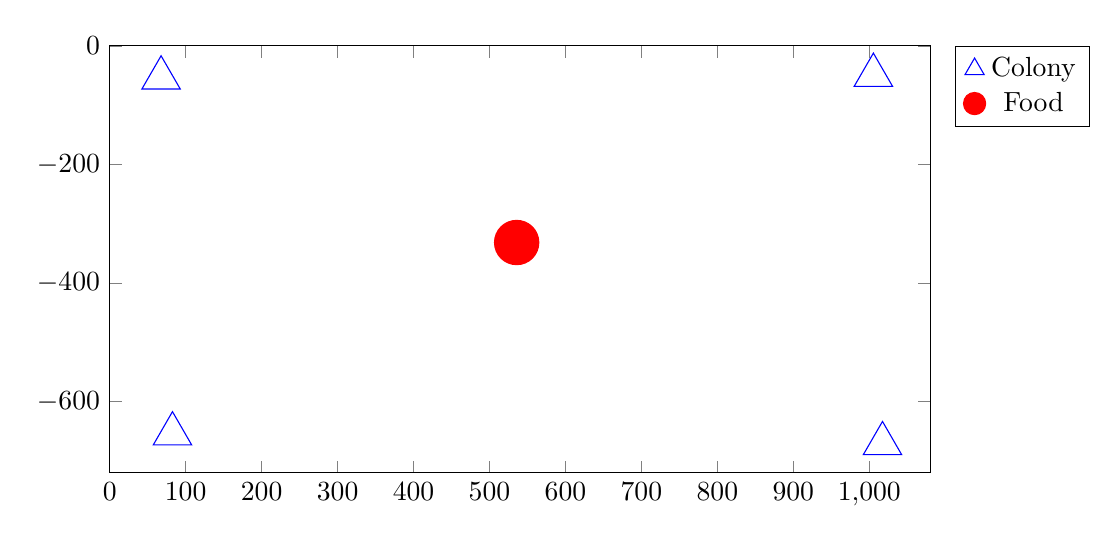
\begin{tikzpicture}
    \begin{axis}[xmin=0, xmax=1080, ymin=-720, ymax=0, width=12cm, height=7cm, legend pos=outer north east, legend image post style={scale=0.5}]

    \addplot[only marks, mark=triangle, mark size=8pt, blue] coordinates {
    (82.63,-654.799) (67.626,-54.18899999999999) (1005.371,-49.684) (1017.374,-671.316) 
    };
    \addlegendentry{Colony}

    \addplot[only marks, mark=*, mark size=8pt, red] coordinates {
    (535.748,-331.971) 
    };
    \addlegendentry{Food}

    \addplot[only marks, mark=square, mark size=8pt, black] coordinates {
    
    };
    \addlegendentry{Obstacle}

    \end{axis}
    \end{tikzpicture}

    \end{document}
    